%
%
%%Text ist für mich noch nicht zufriedenstellend
%In diesem Kapitel geht es um die \emph{Richtcharakteristik von kreisf\"ormigen Antennen}.
%Vorweg genommen bekommt man die \emph{Besselfunktion} als L\"osung.
%Die Herleitung ist aber allgemein f\"ur aller zylindrische K\"orper anwendbar.
%F\"ur das bessere Verst\"andnis wird zuerst der Weg von einer rechteckigen Pauke zu einer kreisf\"ormigen Pauke gemacht und erst danach kommen wir zum Thema \emph{Richtcharakteristik von kreisf\"ormigen Antennen}.
%
%
%
%Potenzreihenherleitung
\section{Potenzreihenherleitung der Besselfunktion}
Das Ziel dieses Abschnittes ist, die Besselfunktion mit der Potenzreihen-Methode die in Kapitel \ref{section:potenzreihen:verallgemeinert} erl\"autert wurde, herzuleiten.
\dots \\
%Dieser Abschnitt befasst sich mit der Potenzherleitung der Besselfunktion. 
%Bei der Herleitung werden Methoden, die in den vorherigen Kapitel  erl\"autert wurden, 
%verwendet. Zuerst m\"uss eine Differenzialgleichung aufgestellt werden.
%Die Besselfunktion kommt aus der Wellengleichung.
%
\dots So kommt man auf die Gleichung \ref{eq:bessel_dgl}, welche grosse \"Ahnlichkeit mit der Gleichung \ref{potenzreihen:verallgemeinert-bessel} aufweisst.
%Die Differenzialgleichung f\"ur die Besselfunktion lautet wiefolgt:
\begin{align}
	r^2 \, R'' \left( r \right)
	+
	r \, R' \left( r \right)
	+
	\left( r^2 - n^2 \right) \, R \left( r \right)
	=
	0
	\label{eq:bessel_dgl}
\end{align}
Im Folgenden wird nun die Gleichung \ref{eq:bessel_dgl}, mithilfe der Potenzreihen-Methode aus dem Kapitel \ref{section:potenzreihen:verallgemeinert}, gel\"ost und der L\"osungsweg aufgezeigt.
\subsection*{Vorgehensweise}
\begin{enumerate}
	\item Die Potenzreihe und deren Ableitungen berechnet.
	\item Die Potenzreihen in die Differenzialgleichung \ref{eq:bessel_dgl} eingesetzen, um
	\item die Indexgleichung f\"ur $\varrho$ zu l\"osen, welche
	\item eine Rekursion der Koeffizienten erm\"oglicht.
	\item Bestimmen der Koeffizienten f\"ur
	\item die Besselfunktion mit ganzzahlige Parametern \ref{eq:bessel_summenformel}.
%	\item Allgemeine Besselfunktion \ref{eq:bessel_summenformel:allgemein}
\end{enumerate}


%Um die Differenzialgleichung zu l\"osen, w\"ahlen wir den Potenzreihenansatz mit der folgenden Potenzreihe und deren Ableitungen:
\subsection*{Potenzreihe und deren Ableitungen}

\begin{normalsize}
	Zum l\"osen der Differenzialgleichung \ref{eq:bessel_dgl} w\"ahlten wir den Ansatz der Potenzreihen-Methode.
	F\"ur den Ansatz ben\"otigen wir zuerst eine allgemeine Potenzreihe wie \ref{eq:bessel:potenzreihe:allgemein}.
	Da in der Differenzialgleichung die erste und zweite Ableitung darin vorkommen,
	muss man die Potenzreihe noch ableiten, was wiederum eine Potenzreiche ergibt,
	wie \ref{eq:bessel:potenzreihe:ersteableitung} und \ref{eq:bessel:potenzreihe:zweiteableitung} zeigen.
\end{normalsize}
\\
\begin{align}
	R \left( r \right)
	&=
	r^{\varrho}
	\sum_{k=0}^{\infty} a_k \, r^k
	\label{eq:bessel:potenzreihe:allgemein}
\\
	R'\left( r \right)
	&=
	\varrho \, r^{\varrho - 1}
	\sum_{k=0}^{\infty} a_k \, r^k
	+
	r^{\varrho}
	\sum_{k=0}^{\infty} a_k \, k \, r^{k - 1}
	\label{eq:bessel:potenzreihe:ersteableitung}
\\
	R'' \left( r \right)
	&=
	\varrho \, \left( \varrho - 1 \right) \, r^{\varrho - 2}
	\sum_{k=0}^{\infty} a_k \, r^k
	+
	2 \, \varrho \, r^{\varrho - 1}
	\sum_{k=0}^{\infty} a_k \, k \, r^{k - 1}
	+
	r^{\varrho}
	\sum_{k=0}^{\infty} a_k \, k \, \left( k - 1 \right) \, r^{k - 2}	
	\label{eq:bessel:potenzreihe:zweiteableitung}
\end{align}
%\\
%\begin{normalsize}
%	Wie man sieht,
%	wird die Potenzreihe mit zunehmender Ableitung immer gr\"osser und un\"ubersichtlicher.
%	Zudem verringert sich bei jeder Ableitung der Grad der Potenz um 1.
%	Wenn man die Potenz als Stelle nimmt,
%	dann kann man auch sagen,
%	dass sich pro Ableitung,
%	alle Koeffizienten um eine Stelle nach links verschieben.
%	Dank dieser Verschiebung ist es m\"oglich,
%	eine Abh\"anigkeit bzw. eine Rekursion der Koeffizienten zu erreichen.
%	Mit der Rekursion ist es wiederum m\"oglich,
%	nur wenige der Koeffizienten selber zu definieren m\"ussen,
%	was den Freiheitsgrad reduziert und somit die Berechnung vereinfacht.
%	
%%	\begin{description}[style = nextline, leftmargin = \parindent, labelindent = \parindent]
%%	%[style = multiline, labelwidth = 3.5cm, leftmargin = 3.5cm, itemsep = 1cm]
%%		\item[Wieso ist es ein Vorteil, den Freiheitsgrad zu reduzieren?]
%%		\dots Parameter reduzieren \dots Anzahl M\"oglichkeiten reduzieren \dots \\
%%	\end{description}
%		
%\end{normalsize}

\subsection*{Potenzreihen in Differenzialgleichung \ref{eq:bessel_dgl} einsetzen}
%Nun kann man die Potenzreihen in die Differenzialgleichung \ref{eq:bessel_dgl} einsetzen und bekommt dann:

\begin{normalsize}
	Der n\"achste Schritt ist,
	die erhaltenen Potenzreihen in die Differenzialgleichung \ref{eq:bessel_dgl} einzusetzen.
\end{normalsize}

\begin{align*}
	r^2 \, R'' \left( r \right)
	+
	r \, R' \left( r \right)
	+
	\left( r^2 - n^2 \right) \, R \left( r \right)
	=
	0
	\tag{\ref{eq:bessel_dgl}}
\end{align*}
%
\begin{align*}
	\overbrace{
		\varrho \, \left( \varrho - 1 \right) \, r^{\varrho}
		\sum_{k=0}^{\infty} a_k \, r^k
		+
		2 \, \varrho \, r^{\varrho}
		\sum_{k=0}^{\infty} a_k \, k \, r^k
		+
		r^{\varrho}
		\sum_{k=0}^{\infty} a_k \, k \, \left( k - 1 \right) \, r^k
	}^{r^2 \, R''\left( r \right)}
	+ \\
	\underbrace{
		\varrho \, r^{\varrho}
		\sum_{k=0}^{\infty} a_k \, r^k
		+
		r^{\varrho}
		\sum_{k=0}^{\infty} a_k \, k \, r^k
	}_{r \, R' \left( r \right)}
	+ 
	\underbrace{
		r^{\varrho}
			\sum_{k=0}^{\infty} a_k \, r^{k + 2}
		-
		n^2 \, r^{\varrho}
		\sum_{k=0}^{\infty} a_k \, r^k
	}_{\left( r^2 - n^2 \right) \, R \left( r \right)}
	= & \, 0
\end{align*}
\\
%Gleiche Summenzeichen zusammenfassen:
\begin{normalsize}
	Fasst man gleiche Terme zusammen, bekommt man:
\end{normalsize}
\begin{align}
	\left(
	\varrho \, \left( \varrho - 1 \right)
	+ 
	\varrho
	-
	n^2
	\right)
	\, r^{\varrho}
	\sum_{k=0}^{\infty} a_k \, r^k
	+ 
	\left(	
	2 \, \varrho
	+
	1
	\right)
	\, r^{\varrho}
	\sum_{k=0}^{\infty} a_k \, k \, r^k
	+
	r^{\varrho}
	\sum_{k=0}^{\infty} a_k \, k \, \left( k - 1 \right) \, r^k
	+ 
	r^{\varrho}
	\sum_{k=0}^{\infty} a_k \, r^{k + 2}
	= \, 0
	\label{eq:bessel:potenzreihe:dgl:vereinfacht}
\end{align}
%
\subsection*{Indexgleichung f\"ur $\varrho$}
%Nun muss man eine Indexgleichung für die Unbekannte $\varrho$ aufstellen, um diese zu bestimmen.
%\ref{section:potenzreihen:verallgemeinert}
%Dazu eignet sich eine Indexgleichung f\"ur den Koeffizienten $a_0$:
\begin{normalsize}
	Indexgleichung f\"ur $a_0$
\end{normalsize}
\begin{align*}
%	\left( \varrho \, \left( \varrho -1 \right) + \varrho - n^2 \right) \, a_0 &= 0 && \left| :a_0 \right. \\
	\varrho \, \left( \varrho -1 \right) + \varrho - n^2 &= 0 && \left| \text{Ausmultiplizieren} \right. \\
	\varrho ^2 - \varrho + \varrho -n^2 &= 0 && \left| \text{Vereinfachen} \right.\\
	\varrho ^2 - n^2 &= 0 && \left| +n^2 \right.\\
	\varrho ^2 &= n^2 && \left| \sqrt{\centerdot} \right.
\end{align*}
\\
\begin{normalsize}
	Aus der Indexgleichung erh\"alt man $\varrho = \pm n$ und $\varrho = \pm 0 $.
	Nun kann man in der Gleichung \ref{eq:bessel:potenzreihe:dgl:vereinfacht} $n$ f\"ur $\varrho$ einsetzen und kommt dann auf \ref{eq:bessel:potenzreihe:dgl:index:eingesetzt}.
	Die zweite L\"osung $\varrho = 0$ wird im Kapitel \ref{chapter:komplex} behandelt.
\end{normalsize}

%Wir beschr\"anken uns in diesem Kapitel nur mit der L\"oesung $\varrho = \pm n$. Die L\"osung f\"ur $\varrho = \pm 0$ wird im Kapitel \ref{chapter:komplex} genauer behandelt.
%Nun kann man $n$ f\"ur $\varrho$ in die Gleichung einsetzen und erh\"alt:

\begin{align}
	\left(
	n \, \left( n - 1 \right)
	+
	n
	-
	n^2
	\right)
	\, r^{n}
	\sum_{k=0}^{\infty} a_k \, r^k
	+
	\left(	
	2 \, n
	+
	1
	\right)
	\, r^{n}
	\sum_{k=0}^{\infty} a_k \, k \, r^k
	+
	r^{n}
	\sum_{k=0}^{\infty} a_k \, k \, \left( k - 1 \right) \, r^k
	+
	r^{n}
	\sum_{k=0}^{\infty} a_k \, r^{\textcolor{red}{k + 2}}
	= \, 0
	\label{eq:bessel:potenzreihe:dgl:index:eingesetzt}
\end{align}
\\
%Als n\"achstes fasst man alles in eine einzige Summe zusammen und vereinfacht diese:
\begin{normalsize}
	In der Gleichung \ref{eq:bessel:potenzreihe:dgl:index:eingesetzt} bildet man mehrmals die Summe von $k=0$ bis $k \rightarrow \infty$.
	Diese Summen kann man zu einer einzigen Summe zusammenfassen und erh\"alt \ref{eq:bessel:summe:zusammengefasst}.
	Da bei der einen Summe $r^{\textcolor{red}{k+2}}$ und nicht wie bei den restlichen Summe $r^k$ vorkommt,
	muss man beim Zusammenfassen die Grenzen der Summe anpassen (\textcolor{red}{rot} markiert).
	Die Gleichung \ref{eq:bessel:summe:zusammengefasst} kann noch zu \ref{eq:bessel:summe:zusammengefasst:vereinfacht} vereinfacht werden.
\end{normalsize}

\begin{align}
	r^n
	\sum_{\textcolor{red}{k=2}}^{\infty}
	\left(
	n \, \left( n - 1 \right) \, a_k 
	+
	2 \, n \, k \, a_k
	+
	k \, \left( k - 1 \right) \, a_k
	+
	n \, a_k
	+
	k \, a_k
	+
	a_{\textcolor{red}{k - 2}}
	-
	n^2 \, a_k
	\right)
	\, r^k
	= 0 
	\label{eq:bessel:summe:zusammengefasst}
	\\
	\nonumber
	r^n
	\sum_{k=2}^{\infty}
	\left(
	\underbrace{ \cancel{n} \, \left( \cancel{n} - \bcancel{1} \right) \, a_k }_{= \, 0}
	+
	2 \, n \, k \, a_k
	+
	\underbrace{k \, \left( k - \xcancel{1} \right) \, a_k}_{=\, k^2 \, a_k}
	+
	\underbrace{\bcancel{n} \, a_k}_{= \, 0}
	+
	\underbrace{\xcancel{k} \, a_k}_{= \, 0}
	+
	a_{k - 2}
	-
	\underbrace{\cancel{n^2} \, a_k}_{= \, 0}
	\right)
	\, r^k
	= 0 
	\\
	r^n
	\sum_{k=2}^{\infty}
	\left(
	2 \, n \, k \, a_k
	+
	k^2 \, a_k
	+
	a_{k - 2}
	\right)
	\, r^k
	= 0
	\label{eq:bessel:summe:zusammengefasst:vereinfacht}
\end{align}
\\
%Weil $r \neq 0$ sein muss, muss $ \left( 2 \, n \, k + k^2 \right) \, a_k + a_{k - 2} = 0$ sein.
%Nun kann man eine Rekursion der Koeffizienten $a_k$ berechnen.
%%
%	\dots Nun muss entweder $r = 0$ sein,
%	damit die Gleichung \ref{eq:bessel:summe:zusammengefasst:vereinfacht} stimmt,
%	oder der Klammerausdruck in der Summe.
%	Da es sinnlos w\"ahre, wenn $r = 0$ ist,
%	was bedeuten w\"urde,
%	dass der Radius $0$ ist,
%	setzten man den Klammerausdruck gleich $0$ und bekommt so f\"ur die Koeffizienten eine Rekursion \ref{eq:bessel_koeffreq}.
\begin{normalsize}
	Damit die Gleichung \ref{eq:bessel:summe:zusammengefasst:vereinfacht} stimmt,
	muss der linke Teil der Gleichung ebenfalls $0$ ergeben.
	Ein Spezialfall,
	der diese Bedingung erf\"ullen w\"urde,
	ist $r = 0$.
	Dieser Spezialfall ergibt jedoch keine Rekursion der Koeffizienten und somit keine L\"osung f\"ur das Problem.
	Demzufolge muss der Ausdruck in der Klammer $0$ ergeben.
	Um eine Rekursion der Koeffizienten zu erhalten,
	setzt man den Ausdruck in der Klammer gleich $0$ und l\"ost die erhaltene Gleichung nach $a_k$ auf.
\end{normalsize}

\begin{align*}
	2 \, n \, k \, a_k
	+
	k^2 \, a_k
	+
	a_{k - 2}
	= 0
	&\Leftrightarrow
	\left(
	2 \, n \, k 
	+
	k^2 
	\right)
	\, a_k
	+
	a_{k - 2}
	= 0 \\
	\Leftrightarrow
	k \,
	\left(
	2 \, n
	+
	k
	\right)
	\, a_k
	= -a_{k - 2}
	&\Leftrightarrow
	\text{Rekursion der Koeffizienten \ref{eq:bessel_koeffreq}}
\end{align*}
\begin{align}
	a_k
	=
	\frac
	{
		-a_{k - 2}
	}{
		k \, \left( 2 \, n + k \right)	
	}
	\label{eq:bessel_koeffreq}
\end{align}
\\
%Da $k \geq 0$ sein muss, sind nur gerade Koeffizienten m\"oglich. Somit kann man f\"ur $k$ nun $2k$ in die Gleichung \ref{eq:bessel_koeffreq} einsetzen und erh\"alt:
%%
%\dots nur gerade Koeffizineten m\"oglich \dots alle Abh\"angig von $a_0$
\begin{normalsize}
	
\end{normalsize}
\begin{align}
	\nonumber
	a_{2k}
	&=
	\frac
	{
		-a_{2k - 2}
	}{
		2k \, \left( 2 \, n + 2k \right)	
	}
	=
	\frac
	{
		-a_{2k - 2}
	}{
		4k \, \left( n + k \right)	
	} 
	=
	\frac
	{
		-a_0
	}{
		4^k \, {k}! \, {\left( n + k \right)}!
	}\\
	&= 
	\frac
	{
		-a_0
	}{
		2^{2k} \, {k}! \, {\left( n + k \right)}!
	}
\end{align}

%Setzt man nun f\"ur $a_0 = \frac{1}{2^n \, {n}!}$ ein, so kommt man auf die Form:

\begin{align}
	J_n \left( r \right)
	&= \nonumber
	\sum_{k=0} ^{\infty}
	\frac
	{
		\left( - 1 \right) ^k \, r ^{2k+n}
	}{
		2^{2k+n} \, {k}! \, { \left( k + n \right) }!
	}
	=
	\sum_{k=0} ^{\infty}
	\frac
	{
		\left( - 1 \right) ^k \, 
		\frac
		{
			r ^{2k+n}
		}{
			2^{2k+n}
		}
	}{
		{k}! \, { \left( k + n \right) }!
	} \\
	&=
	\sum_{k=0} ^{\infty}
	\frac
	{
		\left( - 1 \right) ^k \, 
		\left(		
		\frac
		{
			r
		}{
			2
		} \right) ^{2k+n}
	}{
		{k}! \, { \left( k + n \right) }!
	}
	\label{eq:bessel_summenformel}
\end{align}

%%	Die Gleichung ist für ganzzahlige Koeffizienten.
%%	Übergang zu Gammafunktion erläutern für allgemeine Formel
%$\Gamma \left( \alpha \right) = {\left( \alpha - 1 \right) }!$
%\begin{align}
%	J_{\pm n} \left( r \right)
%	&=
%	\sum_{k=0} ^{\infty}
%	\frac
%	{
%		\left( - 1 \right) ^k \, 
%		\left(		
%		\frac
%		{
%			r
%		}{
%			2
%		} \right) ^{2k+n}
%	}{
%		{k}! \, \Gamma \left( k + n + 1 \right)
%	}
%	\label{eq:bessel_summenformel:allgemein}
%\end{align}


\begin{figure}
	\begin{center}
		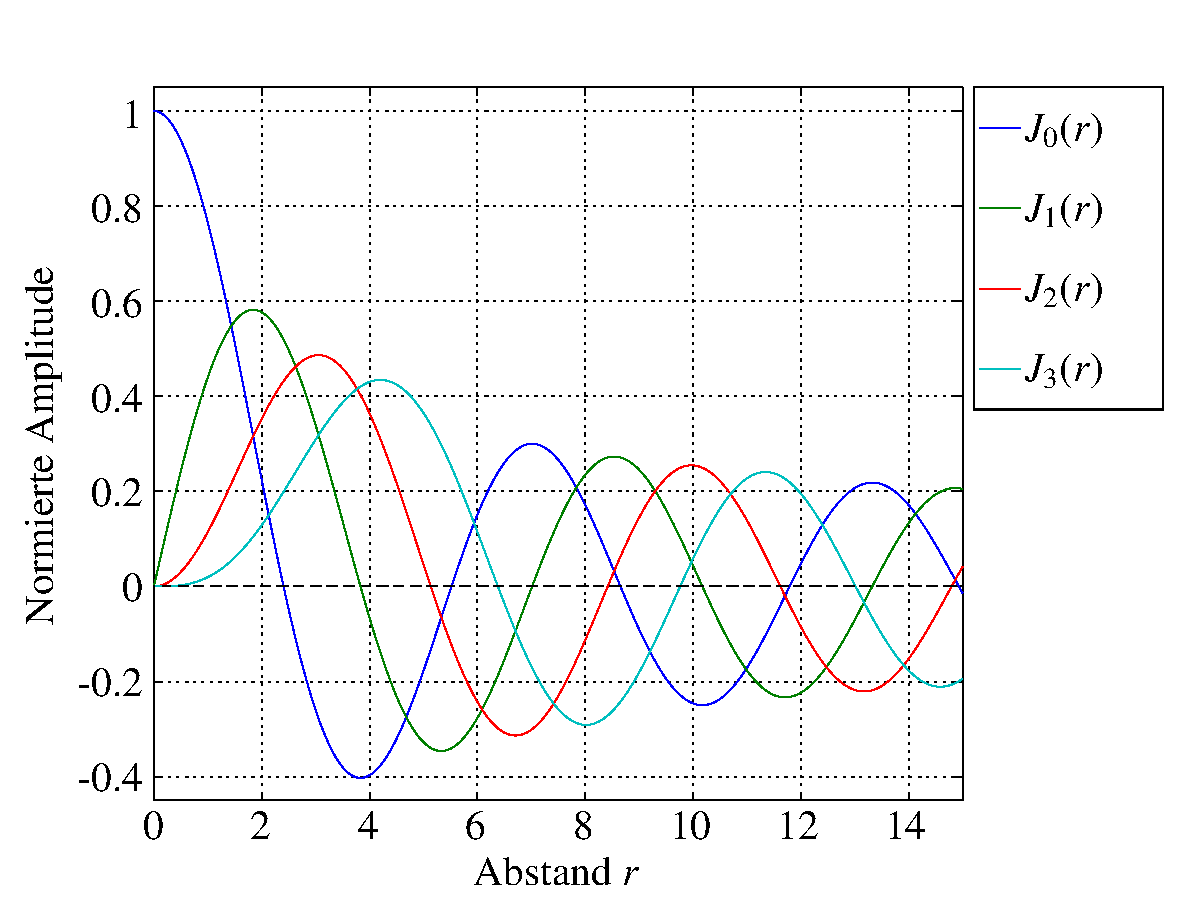
\includegraphics[scale=0.5]{kreis/besselfunction.pdf}
		\label{img:besselfunction}
		\caption[Besselfunktion]{Besselfunktion geplottet}
	\end{center}
\end{figure}

%\newpage
%
%\subsection{Veranschaulichung der Besselfunktion mit Beispielen}
%\begin{itemize}
%	\item Lautsprecher
%	\item Antenne
%	\item Lichtbrechung im Fernglas
%	\item \dots
%\end{itemize}